\documentclass[tikz,border=2pt]{standalone}
\usepackage{amsmath}
\usetikzlibrary{arrows.meta}
\begin{document}
% Call stack of tri(4) with tri(k) = k + tri(k - 1), tri(0) = 0: calls go down to the base case,
% then the values 0, 1, 3, 6, 10 are returned back up.
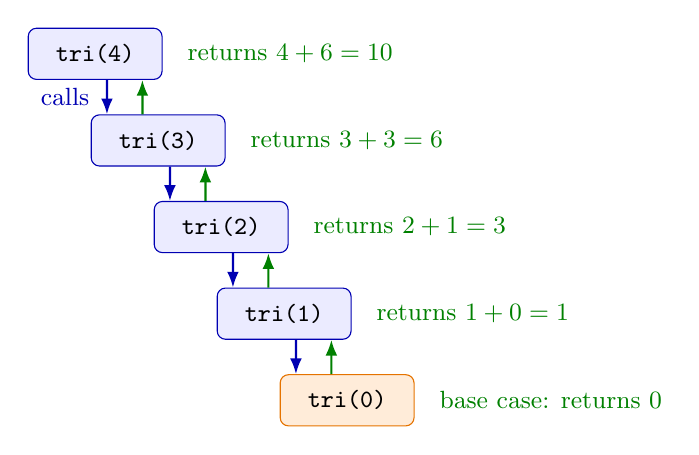
\begin{tikzpicture}[font=\small, >={Latex[length=2mm]},
  call/.style={draw=blue!70!black, fill=blue!8, rounded corners=3pt, minimum width=1.7cm, minimum height=6.5mm, font=\small\ttfamily}]
  \foreach \k [count=\i from 0] in {4,3,2,1} {
    \node[call] (c\i) at (0.8*\i,-1.1*\i) {tri(\k)};
  }
  \node[call, draw=orange!90!black, fill=orange!15] (c4) at (3.2,-4.4) {tri(0)};
  \foreach \i [evaluate=\i as \j using int(\i+1)] in {0,...,3} {
    \draw[->, thick, blue!70!black] ([xshift=1.5mm]c\i.south) -- ([xshift=-6.5mm]c\j.north);
    \draw[->, thick, green!50!black] ([xshift=-2mm]c\j.north) -- ([xshift=6mm]c\i.south);
  }
  \node[anchor=west, green!50!black] at (4.25,-4.4) {base case: returns 0};
  \node[anchor=west, green!50!black] at (3.45,-3.3) {returns $1+0=1$};
  \node[anchor=west, green!50!black] at (2.65,-2.2) {returns $2+1=3$};
  \node[anchor=west, green!50!black] at (1.85,-1.1) {returns $3+3=6$};
  \node[anchor=west, green!50!black] at (1.05,0) {returns $4+6=10$};
  \node[blue!70!black, anchor=east] at (0.05,-0.55) {calls};
\end{tikzpicture}
\end{document}
